\section{A decision that changes with spend}
The 14B-to-32B AIME gate gives a direct check on what it means to match budgets. On the 24 held-out questions the 14B model scores 50.00\% and uses 12,002 output tokens per request. The 32B model scores 60.42\% and uses 12,341. Under independent replay, the gate scores 56.25\% and pays for the first answer plus 3,680 fallback tokens on average. At equal token prices the 32B model alone is both cheaper and more accurate. Even the most favorable question-specific alignment leaves the gate 1.04 points behind (Table~\ref{tab:spend}). At four times the small-model token price, the affordable direct lottery gives a lower score than the independent gate. The direction survives any common reindexing but can change if each question has its own pairing.

\begin{figure}[htbp]\centering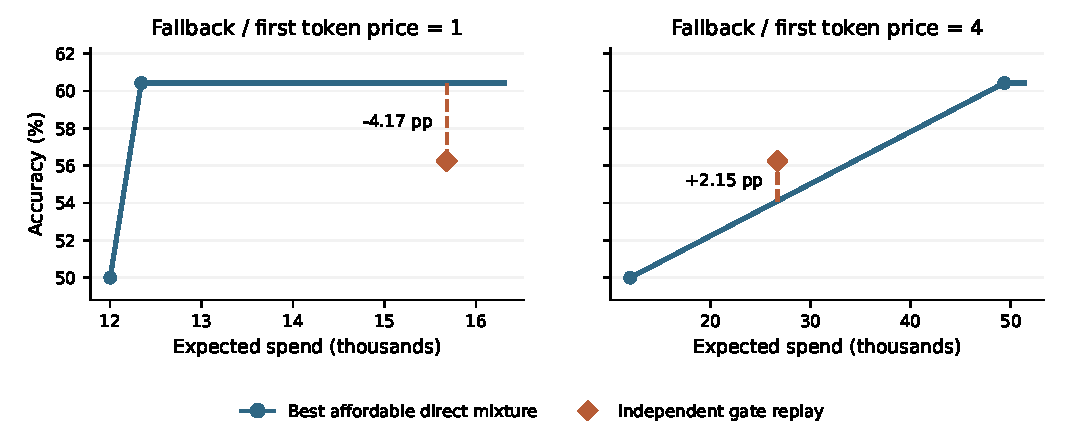
\includegraphics[width=.96\linewidth]{spend.pdf}
\caption{AIME accuracy at two relative output prices. Direct endpoints are the 14B and 32B services. The dashed segment compares the gate with the best direct choice affordable at the gate's own spend. Spend is measured in units of the first model's output-token price.}\label{fig:spend}
\end{figure}

\begin{table}[htbp]\centering\small
\caption{Gate accuracy minus the affordable direct frontier, in percentage points. Common uses a shared draw relabeling and per question permits distinct relabelings. Both intervals include mixtures. The two rows labeled 1, 4 have identical margins at both prices because Nano has the highest standalone score and is affordable throughout.}\label{tab:spend}
\begin{tabular}{lrrrr}
\toprule
Configuration & $\rho$ & Product & Common & Per question \\
\midrule
AIME 14B to 32B & 1 & -4.17 & [-5.21, -2.08] & [-8.33, -1.04] \\
AIME 14B to 32B & 4 & +2.15 & [+0.77, +4.29] & [-2.74, +6.07] \\
MATH Nano to Super & 1, 4 & +0.11 & [-0.04, +0.26] & [-0.06, +0.27] \\
MATH Nano to Llama & 1, 4 & -13.66 & [-14.19, -13.08] & [-15.09, -12.48] \\
\bottomrule
\end{tabular}

\end{table}

For AIME the independent replay crosses zero at $\rho=1.93315$. The first favorable common pairing crosses at 1.52196, and even the least favorable common pairing wins above 2.73414. With question-specific pairing the first crossing falls to 1.32608, while some attainable pairing loses at every finite price. The decision boundary is descriptive and was investigated after observing the reversal at the two planned prices. It is specific to these models, questions and decoding configurations.

\paragraph{Question mix versus response dependence.}
The pairing intervals condition on the question set. To examine a second source of uncertainty, we resampled whole held-out questions 5,000 times, retaining all draws per question and the original calibration cutoff. Each resample recomputed the matched call rate, direct endpoints, and expected spends. The central 95\% of AIME product differences was $[1.25,7.29]$ points at the matched call rate and $[-13.54,4.17]$ points at equal token prices. In 4,105 of 5,000 draws (82.1\%), a positive call-matched difference became negative at equal spend. Refitting on 200 alternative six-question calibration sets reproduced this reversal on 170 complementary test sets. At $\rho=4$ the product bootstrap range was $[-2.00,5.98]$. The fixed archive establishes a reversal under every allowed pairing at equal prices. Its question count leaves the direction on new questions uncertain. These post hoc ranges condition on the original generations and summarize the indicated resampling schemes.

On MATH-500, Nano to Super gained 0.164 points over call-matched random escalation, with a question-bootstrap range $[-0.17,0.50]$. Extra fallback tokens per request were more stable, with a product estimate of 1,142 and bootstrap range $[926,1365]$. At least 1,024 extra fallback tokens were required under every alignment of the original test set. In the equal-spend comparison the product advantage is only 0.112 points and both alignment conventions admit a loss. Replacing Super with Llama yields a loss of at least 12.47 points at both prices. Appendix~\ref{sec:call} reports the additional frozen comparators, a streaming-cost sensitivity and the incomplete 1.5B telemetry.

\section{Do published cascade comparisons change at equal spend?}
The repeated-draw archives permit a sharp pairing analysis for a deliberately simple gate. We also evaluated the budget comparison on published policy measurements from two research groups. Each release supplies five tasks, with CoQA appearing in both. The analyses cover all tasks and published configurations in the specified result files. The releases expose aggregate policy points, so this section evaluates their measured cost and quality directly. It does not infer an unobserved response alignment from those aggregates.

\paragraph{FrugalGPT.} We used the authors' training and test summary tables for 20 nominal budgets per task \cite{frugal}. For each cascade point we first gave the direct comparator the same services eligible for cascade training (five, or six on OVERRULING), and its realized test spend. Of 100 labeled rows, 99 had a strict advantage over the best affordable single model. All 99 survived interpolation between direct services. Repeated budgets often chose the same operating point. Deduplicating within task gives 21 gains and one tie among 22 distinct test cost--score pairs. Thirteen exceed one point, concentrated on three tasks (Table~\ref{tab:external}). Thirteen even exceed the best eligible direct score when its cost constraint is removed, eight by more than one point. Allowing all ten reported services retains 21 strict equal-spend gains, twelve exceeding one point.

\begin{table}[htbp]\centering\small
\caption{FrugalGPT test gains over an affordable query-independent mixture of training-eligible direct services. Counts are distinct within-task cost--score coordinates. Each task's configurations share its test questions.}\label{tab:external}
\begin{tabular}{lrrrr}
\toprule
Task & Distinct & Positive & $>1$ point & Range (points) \\
\midrule
AGNEWS & 5 & 5 & 0 & [0.05, 0.69] \\
CoQA & 4 & 3 & 3 & [0.00, 4.51] \\
HEADLINES & 6 & 6 & 5 & [0.93, 2.51] \\
OVERRULING & 2 & 2 & 0 & [0.11, 0.23] \\
SciQ & 5 & 5 & 5 & [2.55, 5.13] \\
\bottomrule
\end{tabular}

\end{table}

A retrospective test envelope can tune its weights to realized test costs and scores. To obtain a deployable comparator we instead chose mixture weights using only training costs and scores at each original nominal budget, then froze the weights for testing. Both the cascade and the frozen comparator met their nominal budgets on 91 of 100 labeled rows. The cascade exceeded its budget on three, all on OVERRULING. The frozen comparator weakly improved both cost and score, with one strict improvement, on just one row (CoQA, equal score at lower cost). These counts describe the released operating points. Repeated settings and the absence of paired per-item outcomes preclude treating the rows as independent replications.

\paragraph{AutoMix.} We examined the three published procedure families (POMDP, Threshold and SelfConsistency), using all ten matched calibration seeds for each task \cite{automix}. The authors normalize direct costs to 1 and 50 and include verification in the cascade cost. Let $S$ and $L$ be the small and large direct scores, $\beta=(L-S)/49$, and let $C_k,A_k$ be a procedure's cost and score for seed $k$. Its reported incremental benefit per cost is $(A_k-S)/[(C_k-1)\beta]-1$. With the published mean of this ratio, each family supplies a linear equation in $S,\beta$. We solve two linearly independent equations per task, then check the third and all released means, minima, maxima and standard deviations of the ratio. The largest absolute reconstruction discrepancy is below $2\times10^{-14}$.

Drawing a calibration seed uniformly before routing gives the family point $(\bar C,\bar A)$. For each budget in the continuous interval $[1,50]$ we compare three alternatives, each allowed to randomize between one family's point and the two direct services. We integrate the loss from selecting the family with the highest published mean ratio over the piecewise-linear curves, including their intersections. On CoQA, CNLI and QASPER that selection attains the best family envelope at every budget. On QuALITY all three tie with direct service. On NarrativeQA the mean ratio selects Threshold, while SelfConsistency achieves a higher score at all interior budgets. The maximum loss is only 0.141 points at budget 23.01, with a uniform-budget average of 0.057 points. Averaging seed-specific ratios gives different weights to incremental spend than computing a slope from the average point. In a separate seed-by-seed sensitivity, the slope winner incurred a positive loss at some budget in 19 of 50 task--seed cases, with a maximum of 1.46 points on CoQA. Seeds share task test questions. These comparisons quantify the budgeting consequence of using each summary.
